\subsubsection{Interface Mémoire}

Le module de mémoire a été conçu de manière générique à l'aide d'interfaces java. Pour cela elle se décompose en trois parties :

\begin{itemize}
\item l'interface principale de la mémoire, qui déclare les méthodes appelées par les autres modules (Analyse et Raisonnement), et qui est implémentée en tant que mémoire à court terme (ActiveMemory),

\item l'interface de la mémoire épisodique et l'interface de la mémoire sémantique, qui déclarent les méthodes appelées par le module Mémoire.
\end{itemize}

\begin{figure}[H]
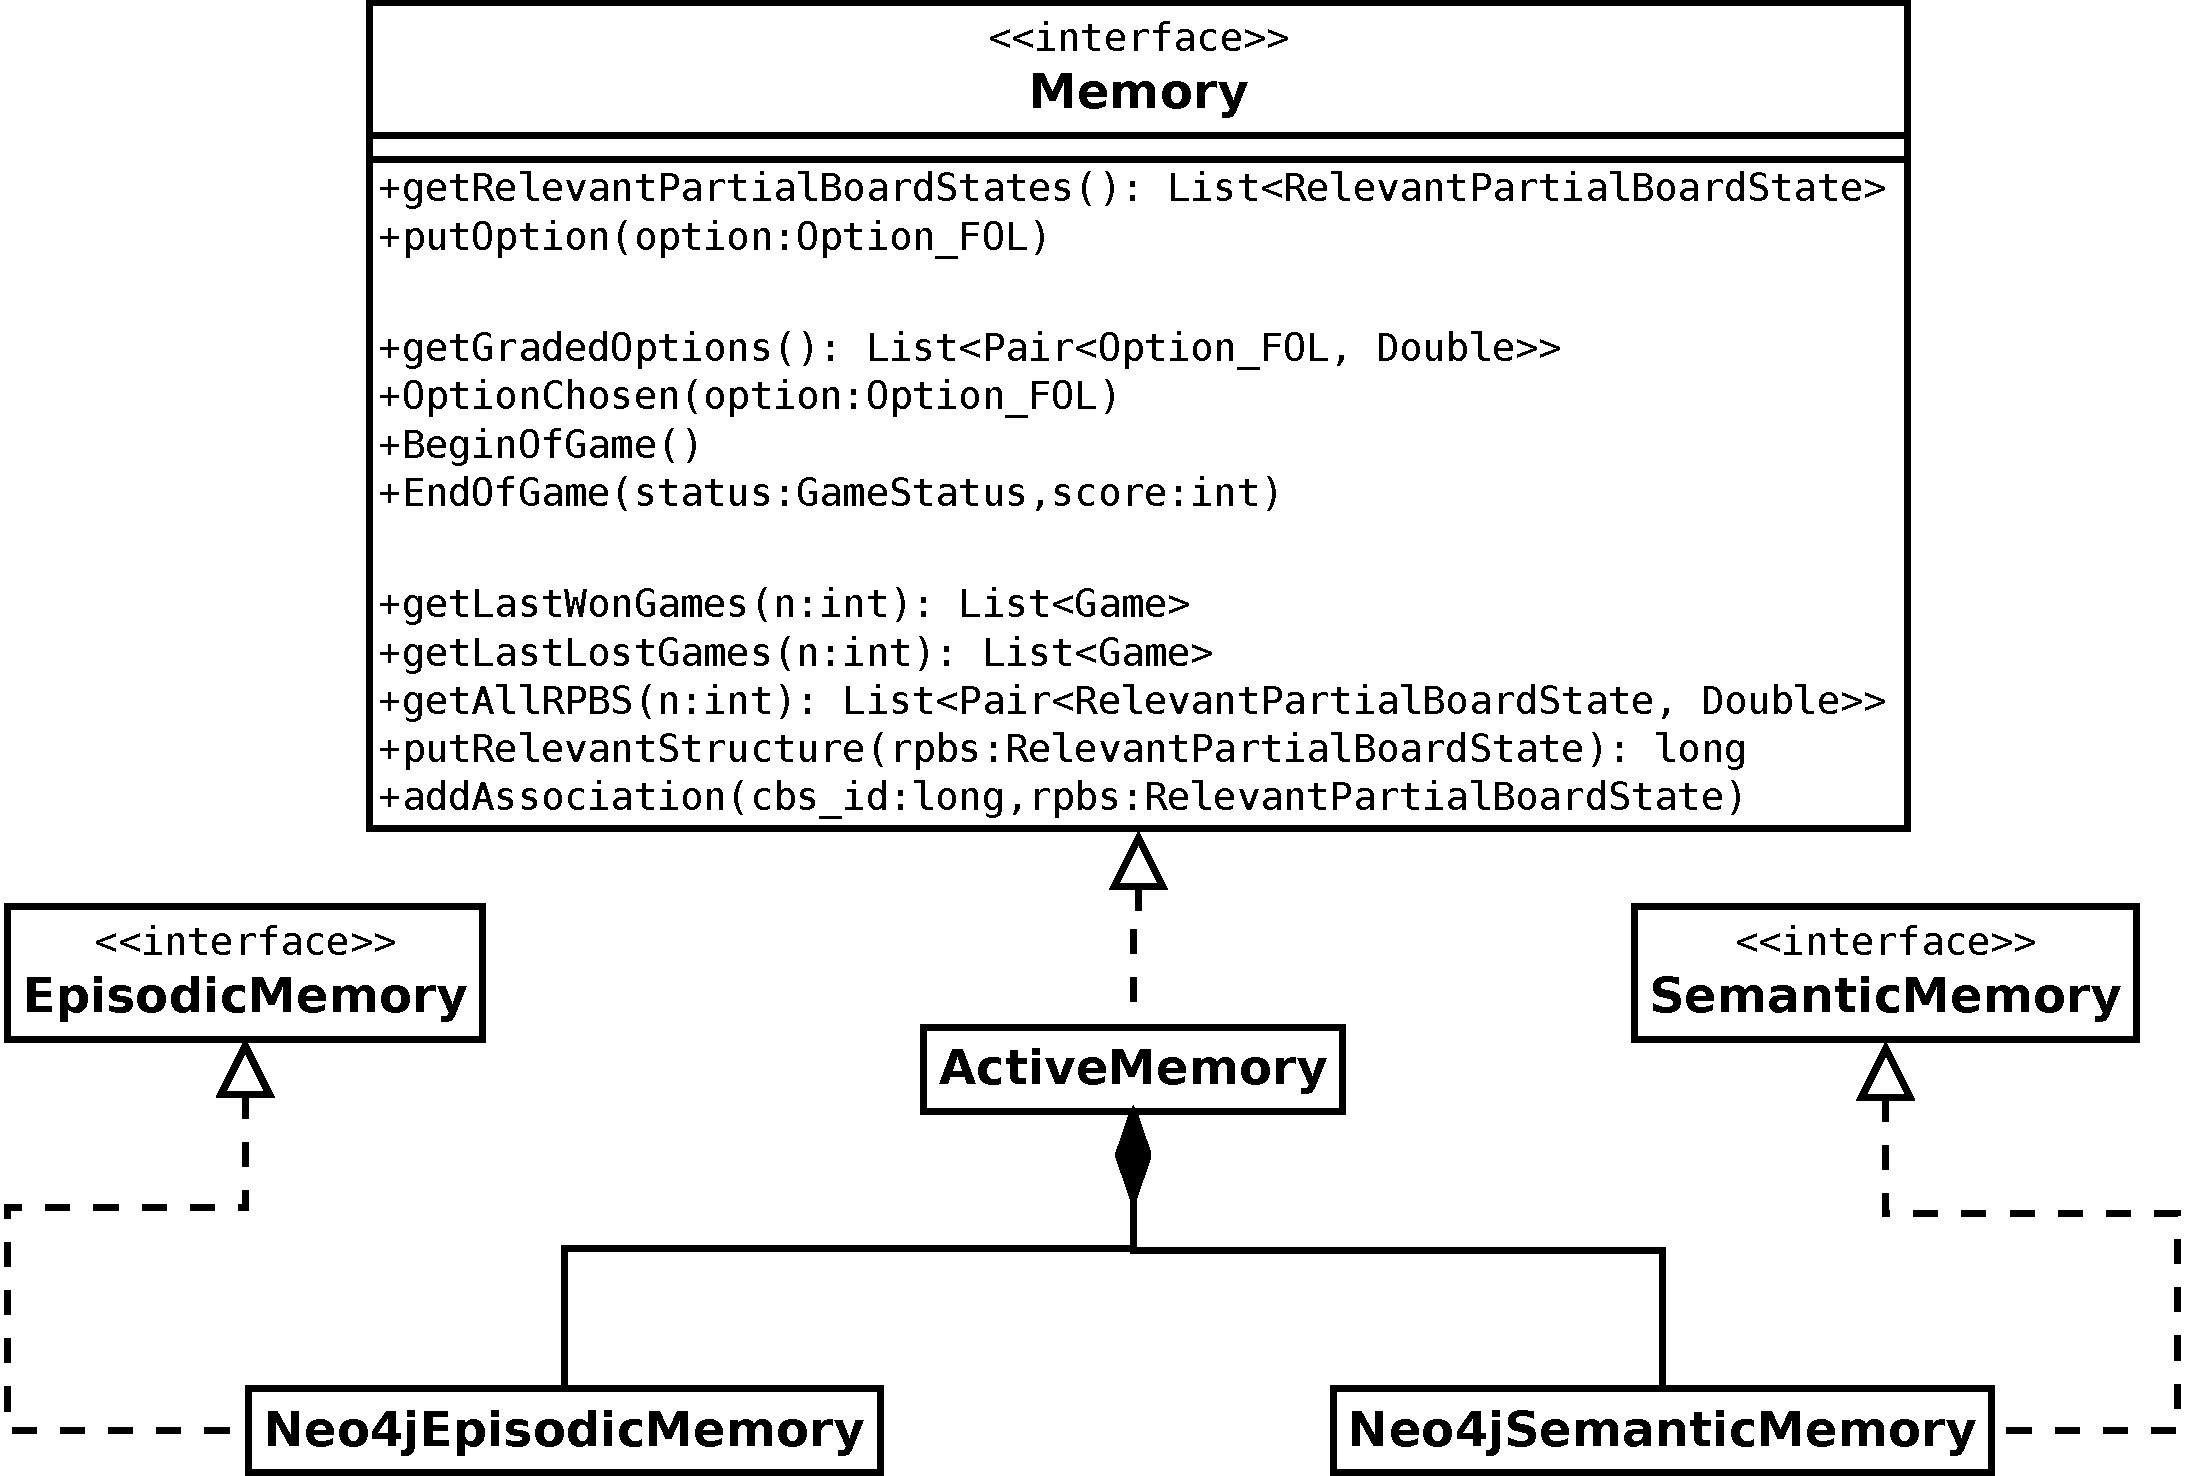
\includegraphics[width=\textwidth]{files/memoire/interface}
\caption{Interface mémoire}
\end{figure}

La mémoire doit également assurer la persistance des données, qui se fait via un module de persistance. Celui-ci est utilisé par une implémentation spécifique des interfaces décrites ci-avant.

\subsubsection{Le \gls{SGBD} Neo4j}

La persistance des données est assurée par un SGBD né de la mouvance \gls{NoSQL} : Neo4j. Il permet la gestion d'une base de données orientée graphe. Nous avons fait le choix d'utiliser un tel système pour plusieurs raisons :

\begin{itemize}
\item nous avions la volonté de découvrir une solution \gls{NoSQL}, que nous n'avons pas eu l'occasion d'étudier lors de notre formation,

\item Neo4j est disponible en plusieurs versions, notamment en version serveur, version webservice REST et version java embarquée. La mémoire n'étant pas accédée de manière concurrente ainsi que pour des soucis de légèreté, c'est la version embarquée (\emph{embedded java})qui a été utilisée,

\item ce type de \gls{SGBD} \gls{NoSQL} permet d'obtenir des temps d'accès plus rapides qu'avec des \gls{SGBD} relationnels traditionnels,

\item la vision graphe de la base de données est adaptée à la conception de notre mémoire\footnote{Notons tout de même qu'il aurait était été possible de stocker les données sous forme de tables},

\item cette solution conserve les propriétés \gls{ACID} des transactions des \gls{SGBD} relationnels traditionnels,

\item la documentation complète et la communauté active permettent de s'initier très rapidement à cette nouvelle technologie,

\item Neo4j est une solution libre distribuée sous licence \gls{GPLv3}.
\end{itemize}

Neo4j étant un \gls{SGBD} \gls{NoSQL} orienté graphe, la base de donnée est représentée sous la forme d'un graphe orienté, composé d'un nœud \og root \fg{}. Chaque nœud et chaque arc peut posséder des attributs. Cependant, il n'est possible de définir que des types d'arc, pour les nœuds on utilise donc une astuce qui consiste en la création d'un \og master\_node \fg{} comme le montre le schéma suivant : 

\begin{figure}[H]
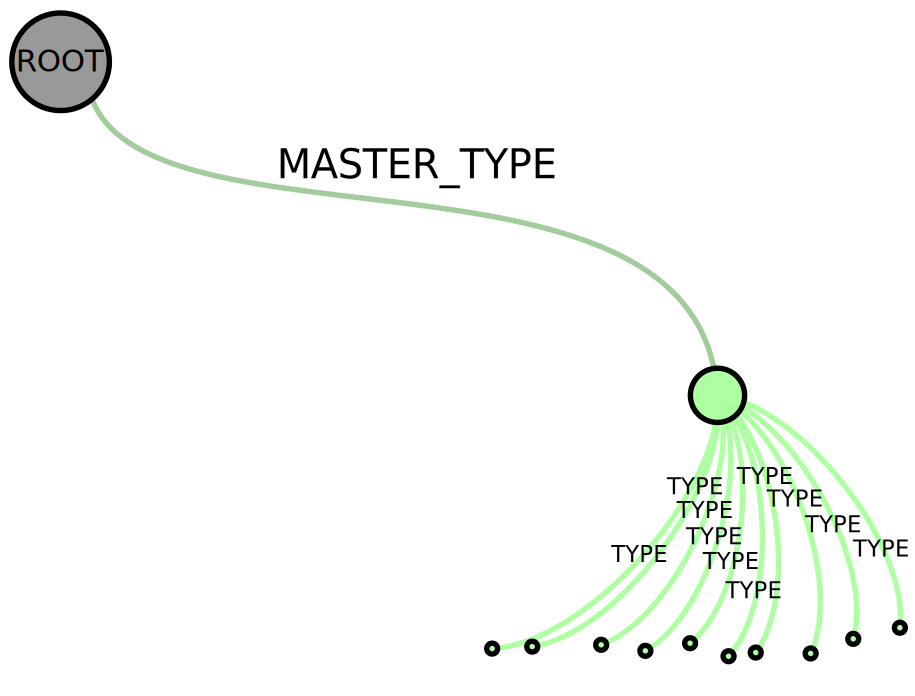
\includegraphics[width=\textwidth]{files/neo4j/example_node_type}
\caption{Exemple de typage des noeuds avec Neo4j.}
\label{example_node_type}
\end{figure}

\subsubsection{Éléments en mémoire}

Le module de persistance permet le stockage de la mémoire épisodique et sémantique, les deux étant liées par les relations entre les \emph{MOVE} et les \emph{CBS}. Nous avons donc besoin des types suivants : 

\textbf{Types de noeud :}
\begin{itemize}
	\item GAME : une partie en mémoire épisodique, 
	\item MOVE : un coup joué en mémoire épisodique,
	\item CBS : un CBS en mémoire sémantique,
	\item RPBS : un RPBS en mémoire sémantique.
\end{itemize}


\textbf{Types de liens :}
\begin{itemize}
	\item Relations maitres
		\begin{itemize}
			\item MASTER\_ATTR,
			\item MASTER\_OBJ,
			\item MASTER\_GAME,
			\item MASTER\_MOVE.
		\end{itemize}
	\item Relations de type
		\begin{itemize}
			\item ATTRIBUTE,
			\item OBJECT,
			\item MOVE,
			\item GAME,
			\item LAST\_GAME (relation GAME spéciale, signifiant que cette partie est la dernière jouée).
		\end{itemize}
	\item Relations en mémoire épisodique
		\begin{itemize}
			\item PREV\_GAME : permet à partir d'une partie d'accéder à la précédente,
			\item LAST\_MOVE : permet à partir d'une partie d'accéder au dernier coup joué,
			\item PREV\_MOVE : permet à partir d'un coup d'accéder au précédent,
			\item STATE\_BOARD : permet de lier un coup à l'état de plateau correspondant.
		\end{itemize}
	\item Relations en mémoire sémantique
		\begin{itemize}
			\item RELATED : décrit la présence d'un RPBS dans un CBS.
		\end{itemize}
	\end{itemize}

\subsubsection{Mémoire épisodique}

La représentation sous forme de graphe se prête parfaitement à la mémorisation des parties et des coups sous la forme d'une double liste chaînée. La figure~\ref{episodic_graph} représente la mémoire épisodique telle qu'elle est stockée dans Neo4j.

On visualise parfaitement les trois \og master\_node \fg{} permettant de typer les \emph{GAME}, \emph{MOVE} et \emph{ATTRIBUTES}. Le parcours des parties se fait via la relation \emph{PREV\_GAME} et celui des coups via la relation \emph{PREV\_MOVE}.

On remarque également que les relations \emph{BOARD\_STATE} permettent de faire la liaison entre la mémoire sémantique et la mémoire épisodique.

\begin{figure}[H]
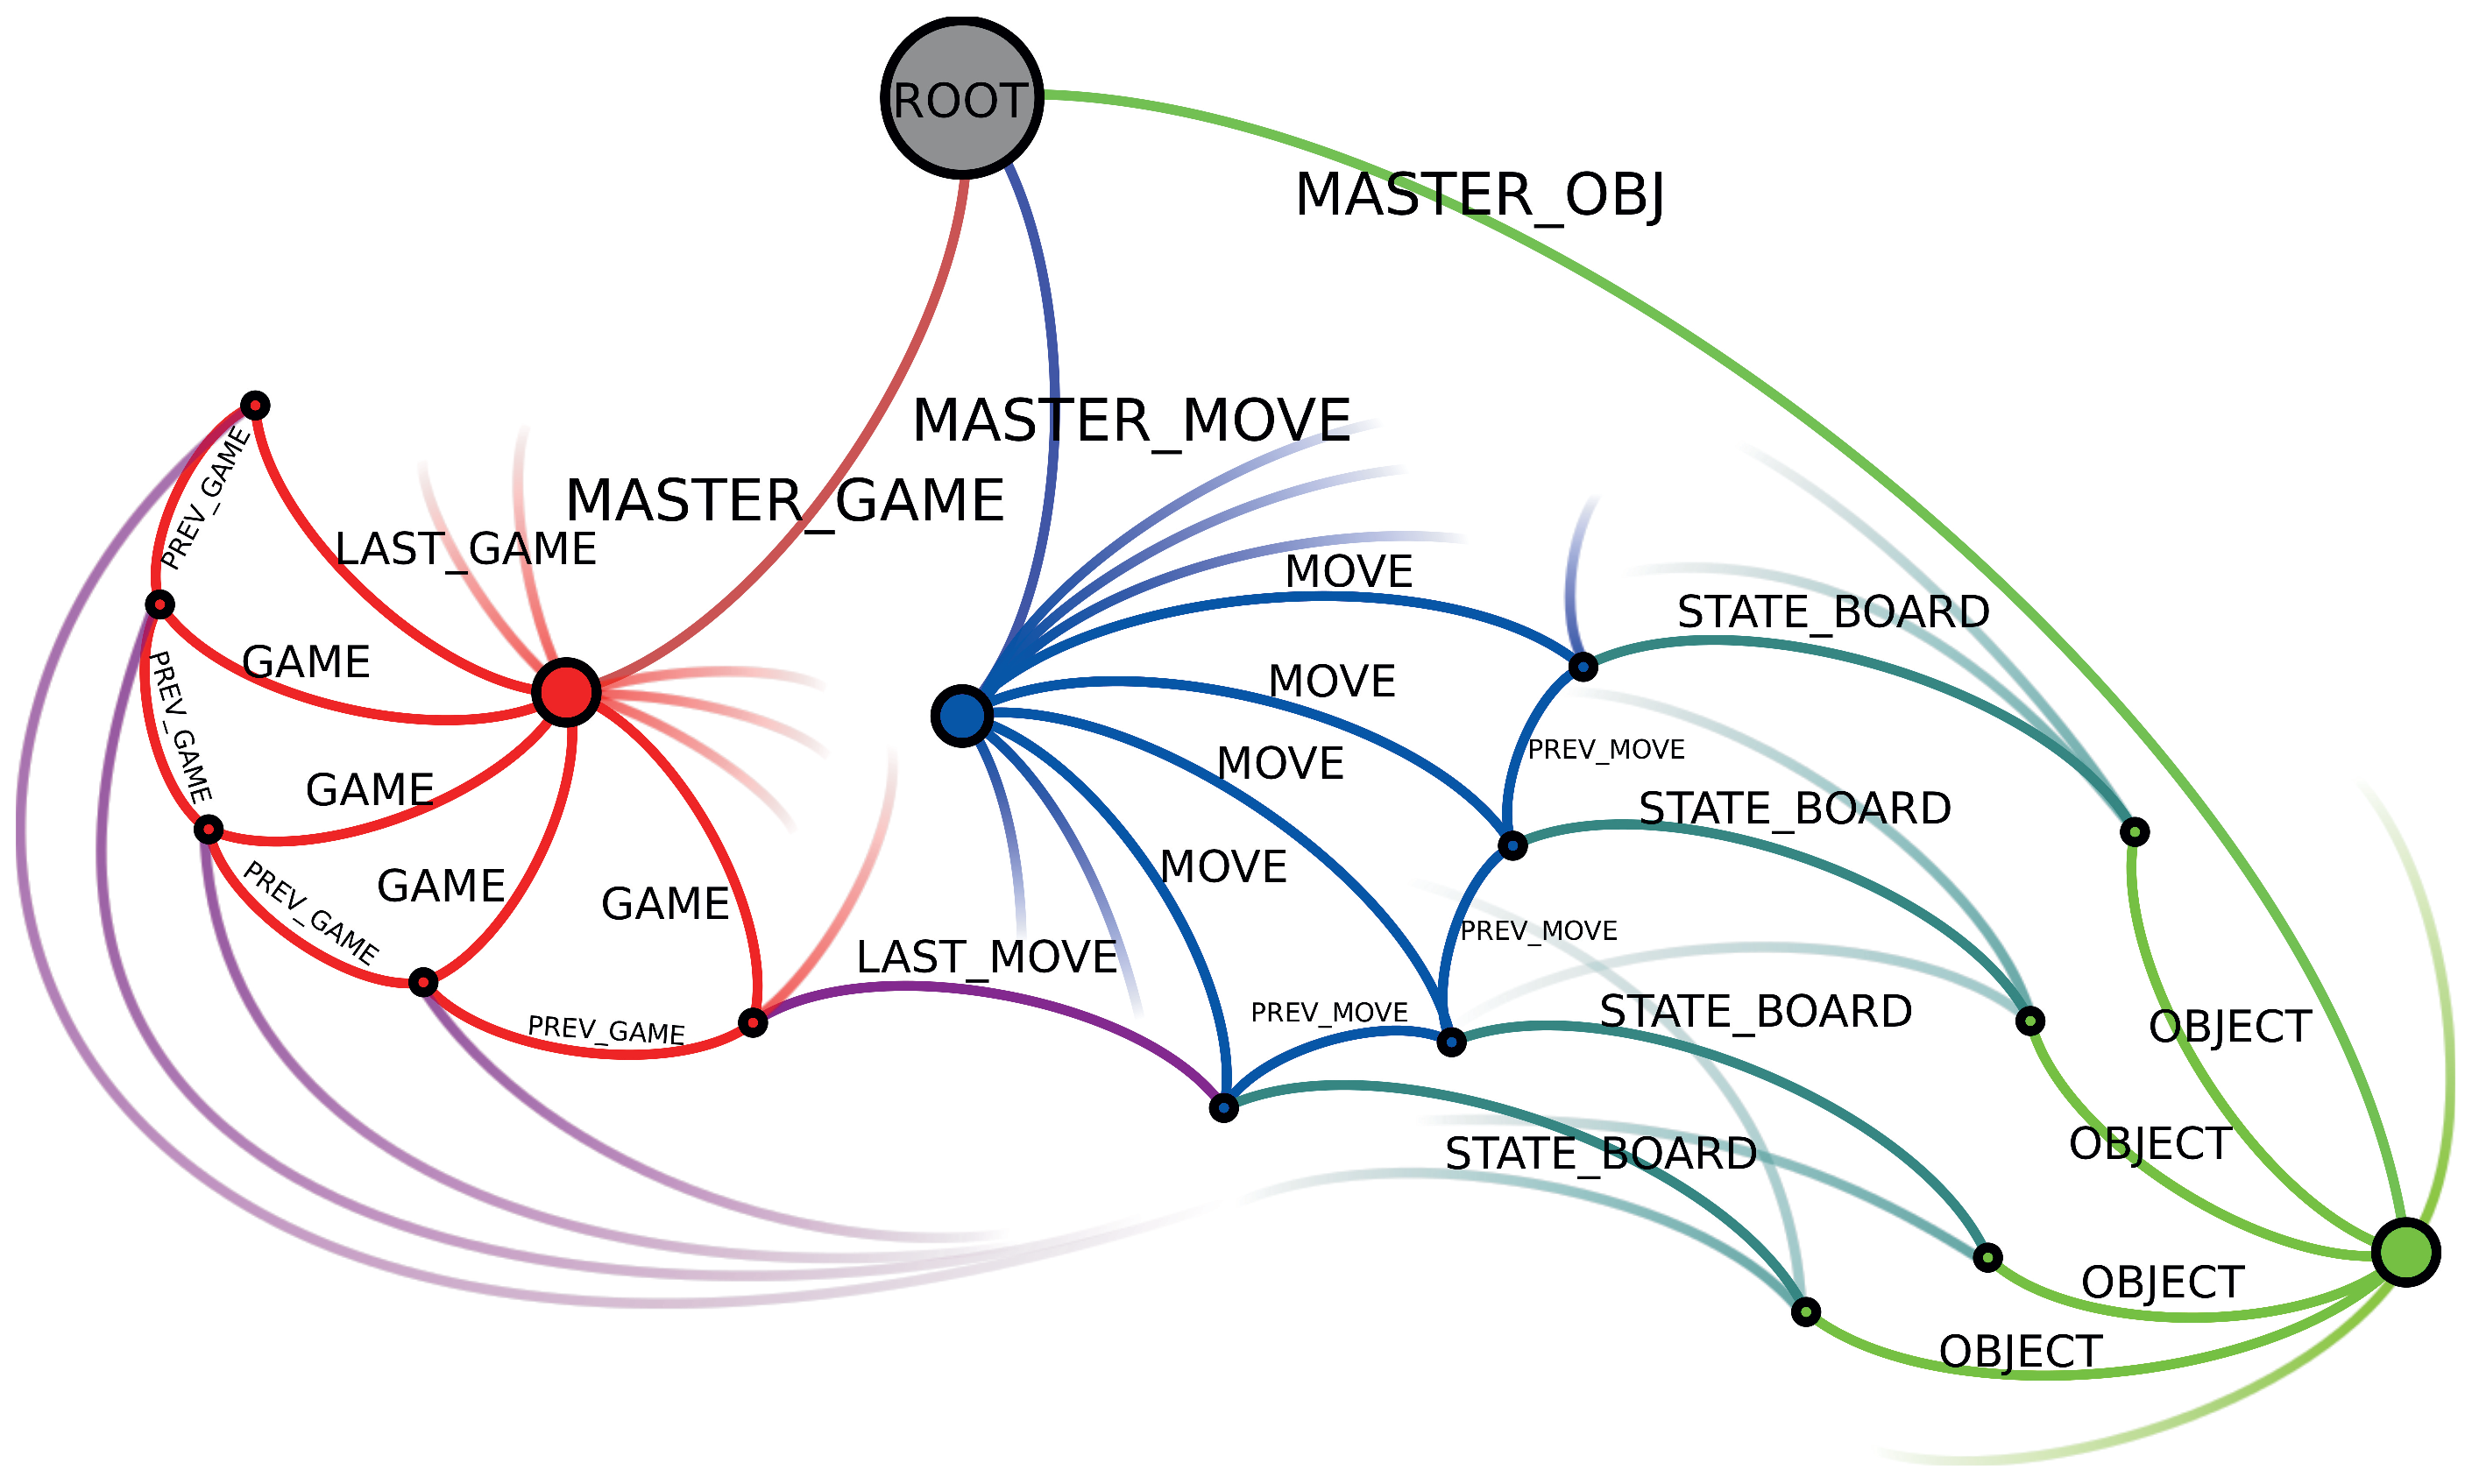
\includegraphics[width=\textwidth]{files/neo4j/episodic_graph}
\caption{Représentation de la mémoire épisodique dans Neo4j.}
\label{episodic_graph}
\end{figure}

\subsubsection{Mémoire sémantique}

Class aptent taciti sociosqu ad litora torquent per conubia nostra, per inceptos himenaeos. Vestibulum arcu massa, hendrerit vel tempor in, sollicitudin in erat. Curabitur non risus nec elit consectetur faucibus sed sed purus. Nam blandit porta ipsum vitae vestibulum. Etiam imperdiet, orci sit amet tincidunt faucibus, urna diam porttitor mauris, at auctor metus neque at nibh. Morbi vel elit venenatis mauris rutrum vehicula. Nam scelerisque iaculis suscipit. Quisque pretium euismod ipsum at elementum. Vestibulum sit amet elit fringilla mauris cursus tincidunt eget sed ante. Ut laoreet ultricies lacus, sed aliquam enim rhoncus ut. Aliquam erat volutpat. Donec ac nulla massa. Maecenas laoreet, magna sed congue venenatis, lacus mi luctus elit, sed sagittis justo nisi ut felis. Aliquam interdum, leo non vestibulum euismod, enim eros eleifend ligula, at aliquet mi eros vitae diam. Suspendisse malesuada scelerisque quam at sodales. Fusce ac lacus sed massa pretium bibendum. 

\subsubsection{Gestion de la persistance}

Ut tincidunt blandit venenatis. Praesent vel nibh vel sem viverra eleifend a rhoncus dolor. Praesent vestibulum orci mattis tellus sagittis sit amet sollicitudin elit gravida. Nam dapibus luctus tortor, ut sodales enim ultrices vel. Nulla urna urna, elementum vehicula porta ut, varius ut turpis. Vestibulum iaculis dolor sed est tempus nec imperdiet massa mollis. Ut in dignissim felis. Cras aliquet, turpis vel fermentum sollicitudin, elit
nulla

lobortis neque, ut tristique justo metus quis urna. Integer tincidunt, dolor ac sodales venenatis, metus dui bibendum mi, nec vehicula est neque volutpat libero. Nunc viverra rhoncus neque nec ultricies. Praesent consectetur metus et mi placerat ac fringilla sem congue. Nullam eu nisl in arcu condimentum fringilla. 

Ut tincidunt blandit venenatis. Praesent vel nibh vel sem viverra eleifend a rhoncus dolor. Praesent vestibulum orci mattis tellus sagittis sit amet sollicitudin elit gravida. Nam dapibus luctus tortor, ut sodales enim ultrices vel. Nulla urna urna, elementum vehicula porta ut, varius ut turpis. Vestibulum iaculis dolor sed est tempus nec imperdiet massa mollis. Ut in dignissim felis. Cras aliquet, turpis vel fermentum sollicitudin, elit nulla lobortis neque, ut tristique justo metus quis urna. Integer tincidunt, dolor ac sodales venenatis, metus dui bibendum mi, nec vehicula est neque volutpat libero. Nunc viverra rhoncus neque nec ultricies. Praesent consectetur metus et mi placerat ac fringilla sem congue. Nullam eu nisl in arcu condimentum fringilla. 
